\documentclass[a4paper,12pt]{article}
\usepackage[a4paper,top=1.3cm,bottom=2cm,left=1.5cm,right=1.5cm,marginparwidth=0.75cm]{geometry}
\usepackage{cmap}					
\usepackage[warn]{mathtext} 		
\usepackage[T2A]{fontenc}			
\usepackage[utf8]{inputenc}			 
\usepackage[english,russian]{babel}	
\usepackage{longtable}
\usepackage{float}
\restylefloat{table}
\usepackage{graphicx}
\usepackage{tabularx}
\usepackage{hyperref}
\usepackage[rgb]{xcolor}
\usepackage{amsmath,amsfonts,amssymb,amsthm,mathtools} 
\mathtoolsset{showonlyrefs=true}
\usepackage{euscript}
\usepackage{mathrsfs}
\date{\today}
\begin{document}

\begin{titlepage}
	\begin{center}
		{\large МФТИ}
	\end{center}
	\begin{center}
		{\large ФРКТ}
	\end{center}
	
	
	\vspace{4.5cm}
	{\huge
		\begin{center}
			{\bf ВПВ по оптике}\\
			Духи Лаймана.
		  
		

		\end{center}
	}
	\vspace{9cm}
	\begin{flushright}
		{\LARGE  Добровольская Ксения 
			\vspace{0.2cm}
			Б01-101}
	\end{flushright}
	\vspace{8cm}
	
\end{titlepage}

\section{Аннотация}

  В данной работе наблюдались духи Лаймана - эффект, связанный с неточностью дифракционной решетки (под неточностью подразумевается смещение каждого n - ного штриха решетки на x, относительно своего правильного положения), были измерены длины волн и положения духов, в зависимости от числа n и периода решеток d.
  
  
  В работе использовались: лазерная указка, бумажная линейка, неточные дифракционные решетки, расчерченные лазером на металлической линейке, со следующими параметрами:
  
  
  \begin{table}[H]
\begin{center}
\begin{tabular}{|c|c|c|c|c|}
\hline $N $&$d,$мм&$n $, шт&$x$, мм\\
\hline 1&0.1&5&0.02\\
\hline 2&0.2&5&0.02\\
\hline 3&0.2&3&0.02\\
\hline 4&0.1&5&0.01\\
\hline 5&0.2&5&0.01\\
\hline 6&0.2&3&0.01\\

\hline 
\end{tabular}
\end{center}
\end{table}
  
  
    \begin{figure}[H]
  \begin{center}
    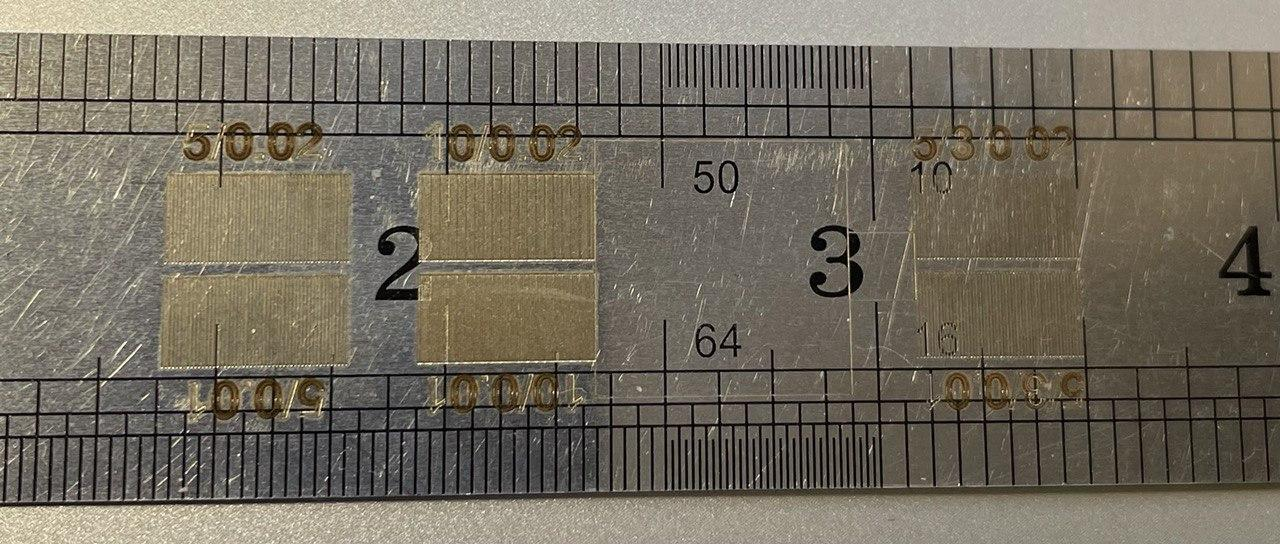
\includegraphics[width=10cm]{ex1.jpg}
    \caption{Схема экспериментальной установки}
    \label{fig:}
  \end{center}
\end{figure}



\section{Теоретическое введение.} 
  
  В идеальной дифракционной решетке все штрихи должны быть идентичны по глубине и форме и расстояния между ними должны быть одинаковы с точностью до малых долей этого расстояния. Так как для изготовления такой решетки требуется точность, значительно превосходящая
точность винторезных станков, то у всех решеток, нарезанных этим способом, обнаруживаются заметные дефекты, в некоторых случаях очень
существенные. К основным дефектам решетки относятся следующие:


1.\textbf{Духи Роуланда} — ложные слабые линии, появляющиеся в спектре
на небольших расстояниях от интенсивных линий. Возникновение линий
связано с периодической нерегулярностью в расположении штрихов
с большим периодом.


2.\textbf{Духи Лаймана} — ложные линии, появляющиеся из-за периодической нерегулярности в расположении штрихов с малым периодом (например, если каждый пятый штрих решетки слегка смещен относительно своего идеального положения, то это соответствует появлению
периодичности, в пять раз превышающей периодичность решетки, что
в свою очередь приводит к появлению «духа», кажущаяся длина волны
которого равна  $\frac{\lambda}{5}$). Такой недостаток решетки может быть связан с регулярной вибрацией делительной машины, нарезающей решетки. Духи Лаймана могут создавать значительные трудности при наблюдении спектров, в особенности сложных.
  


В связи с возможностью изготавливать решетки только с большим периодом (порядка десяти штрихов на миллиметр), в данной работе исследуется влияние только духов Лаймана. 


Дадим математическое объяснение происходящему:


  Решетку с N = mn штрихами можно разбить на m групп, по n штрихов в каждой. Интенсивность в любой точке Р на экране складывается от вкладов m групп, каждая из которых дает вклад
  
  \[I_n = I_0 \frac{sin^2 na}{sin^2 a}\]
  
  , где $a = kdsin^2 \theta/ 2, \theta -$ угол, под которым видна точка Р.
  
  Тогда для вклада от каждой группы имеем:
  
  \[I = I_n \frac{sin^2 ma_1}{sin^2 a_1}\]
  
 , где $a_1 = na$.
 
 В этой суммарной интенсивности имеем ввиду, что при a = $\frac{\pi}{n}, \frac{2\pi}{n}, .... \frac{(n-1)\pi}{n}$ интенсивность отдельной группы $I_n = 0$.
 
 
Предположим, что в расположении n последовательных линий есть такая неравномерность, что решетка из n линий, которую мы считаем повторяющейся m раз, сама по себе является несовершенной решеткой.

Тогда $I_n$ не занулится во всех местах где a = $\frac{\pi}{n}, \frac{2\pi}{n}, .... \frac{(n-1)\pi}{n}$ и эти порядки решетки для каждой из m групп будут видны. 
  
  Далее предположим, что решетка из n линий имеет периодическую ошибку. Для определенности примем, что эта ошибка встречается в каждой третьей строке. То есть каждая третья строка немного смещена, а остальные строки остаются на своих местах. Тогда $I_n$ будет иметь некоторое заметное значение при a = $\frac{\pi}{3}, \frac{2\pi}{3}$.
  
  
  Интенсивность света, заданная всем спектром для длины волны, будет заметна для тех значений a = $\frac{\pi}{n}, \frac{2\pi}{n}, .... \frac{(n-1)\pi}{n}$, которые приближаются к значениям a = $\frac{\pi}{3}, \frac{2\pi}{3}$. Таким образом, будут видны скачки интенсивности в промежутках между главными максимумами дифракционной решетки, что будет создавать впечателение, как будто в исходном свете присутствует компонента с длиной волны $\frac{\lambda}{3}$, а в общем случае $\frac{\lambda}{n}$. Из-за возникновения этой ложной компоненты данный эффект связывают с возникновением духа.
  
  

\section{Экспериментальная установка.} 


  Дифракционные решётки, которые обычно
используются для анализа спектров, имеют порядка
$10^3 - 10^4$ штрихов на сантиметр, т. е. имеют период d,
сравнимый с длиной волны света видимого
диапазона. На грубых решётках (d $>> \lambda $) из-за
малых углов дифракции обнаружить и, тем
более, исследовать дифракционную картину крайне
сложно. В этом случае эффективным оказывается
использование скользящих лучей, когда угол
падения близок к $\frac{\pi}{2}$.

  При наклонном падении лучей на
дифракционную решётку условие дифракционного
максимума m-го порядка имеет вид:


\[d(sin\varphi_0 - sin\varphi_m) = m\lambda  \]


  В дальнейшем мы будем использовать не углы падения , а углы скольжения – $\theta = 90 - \varphi$ .
  Тогда, условие максимума перепишется в виде:


\[d(cos\theta_0 - cos\theta_m) = m\lambda \approx (d sin\theta_0)(\theta_m - \theta_0) \]


  Угловое расстояние между максимумами дифракционной картины:

\[\Delta \theta = (\theta_m - \theta_0) = \frac{\lambda}{d sin\theta_0}  \]

 Видно, что роль эффективного периода решётки в этом случае играет величина $d_1 = d sin\theta_0$,
которая может быть сделана очень малой. Скользящее падение лучей как бы уменьшает период решётки и увеличивает углы дифракции. Таким методом удаётся получать отчётливые дифракционные картины даже от очень грубых решёток.


  Рассчитаем линейное расстояние между дифракционными максимумами в схеме на рис 2.
  
  Координата максимума m-го порядка $x_m = Ltg\theta_m$, а (m + 1)-го порядка $x_{m+1} = Ltg\theta_{m+1}$. Считая углы дифракции мало отличающимся от угла $\theta_0$, соответствующего зеркальному отражению от решётки (m = 0), выразим линейный период дифракционной картины через его угловой размер:



\[\Lambda = x_{m+1} - x_m = L(tg\theta_{m+1} - tg\theta_m) \approx \frac{L}{cos^2 \theta_0} \Delta \theta = \frac{L\lambda}{d cos^2 \theta_0sin\theta_0} \]


  Заметим, что расстояние между максимумами интенсивности прямо пропорционально длине волны света $\lambda$ и обратно пропорционально периоду решетки d.


  \begin{figure}[H]
  \begin{center}
    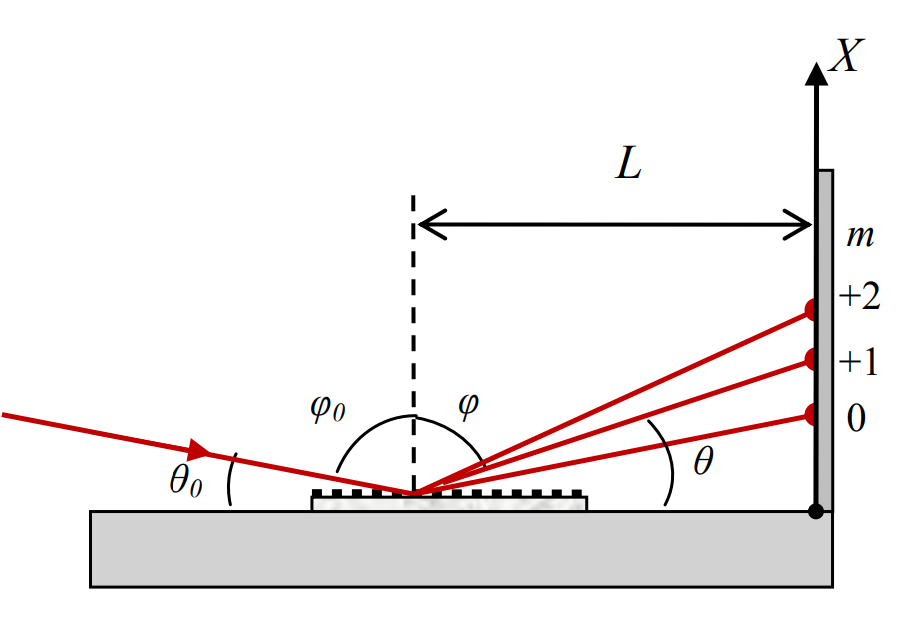
\includegraphics[width=10cm]{ex2.png}
    \caption{Схема экспериментальной установки}
    \label{fig:}
  \end{center}
\end{figure}



\section{Наблюдение и анализ дифракции на различных решетках.} 

Экспериментальная установка приведена на рис. 3.


На расстоянии L = 80 см от экрана расположена дифракционная решетка, а на ней приподнятая на малый угол с помощью бумажной подставки и включенная лазерная указка. На экране приклеена бумажная линейка, помогающая фиксировать расстояния между максимумами. 

  \begin{figure}[H]
  \begin{center}
    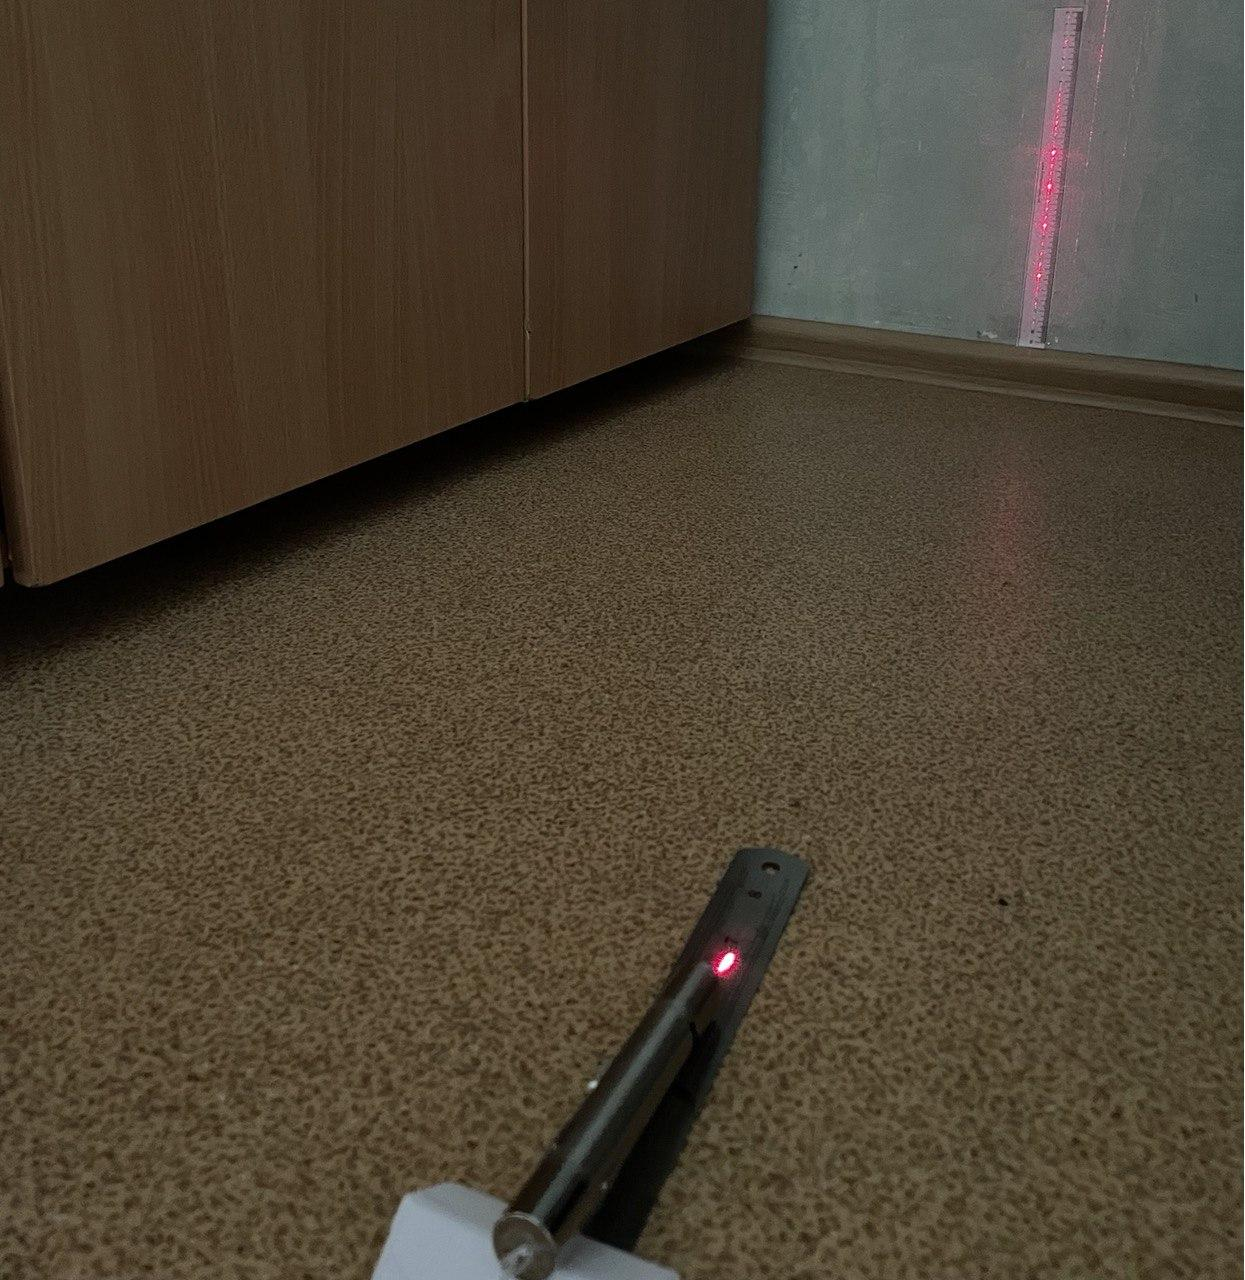
\includegraphics[width=10cm]{ex2.jpg}
    \caption{Экспериментальная установка.}
    \label{fig:}
  \end{center}
\end{figure}



\begin{enumerate}
\item Рассчитаем линейные расстояния между главными максимумами дифракционной картины по формуле из теоретического введения:

\[ \Lambda = \frac{L\lambda}{d cos^2 \theta_0sin\theta_0} = \frac{0.8 * 0.6 * 10^{-6}}{0.01 * 10^{-3} * 1 * 0.1/0.8} \approx 2\]см,

для решетки с периодом 0.02 мм, соответственно в два раза меньше, то есть примерно 1 см.


\item Дифракционная решетка с десятью штрихами на миллиметр и смещением каждого пятого штриха на 0.02 мм дает дифракционную картину изображенную на рис.4. Видно, что расстояния между главными максимумами, как и было получено в теоретическом рассчете, около 2 см, но между каждыми соседними максимумами ярко выражены еще 4 максимума, то есть на один главный максимум приходится пять ложных, что свидетельствует о наблюдении духа Лаймана с длиной волны $\frac{\lambda}{5}$, что согласуется с теоретическим введением.


\item Дифракционная решетка с пятью штрихами на миллиметр и смещением каждого пятого штриха на 0.02 мм дает дифракционную картину изображенную на рис.5. Видно, что расстояния между главными максимумами, действительно в два раза меньше предыдущих и составляет отоко 1 см, причем здесь тоже между каждыми соседними максимумами ярко выражены еще 4 максимума, что опять свидетельствует о наблюдении духа Лаймана с длиной волны $\frac{\lambda}{5}$.

  \begin{figure}[H]
  \begin{center}
    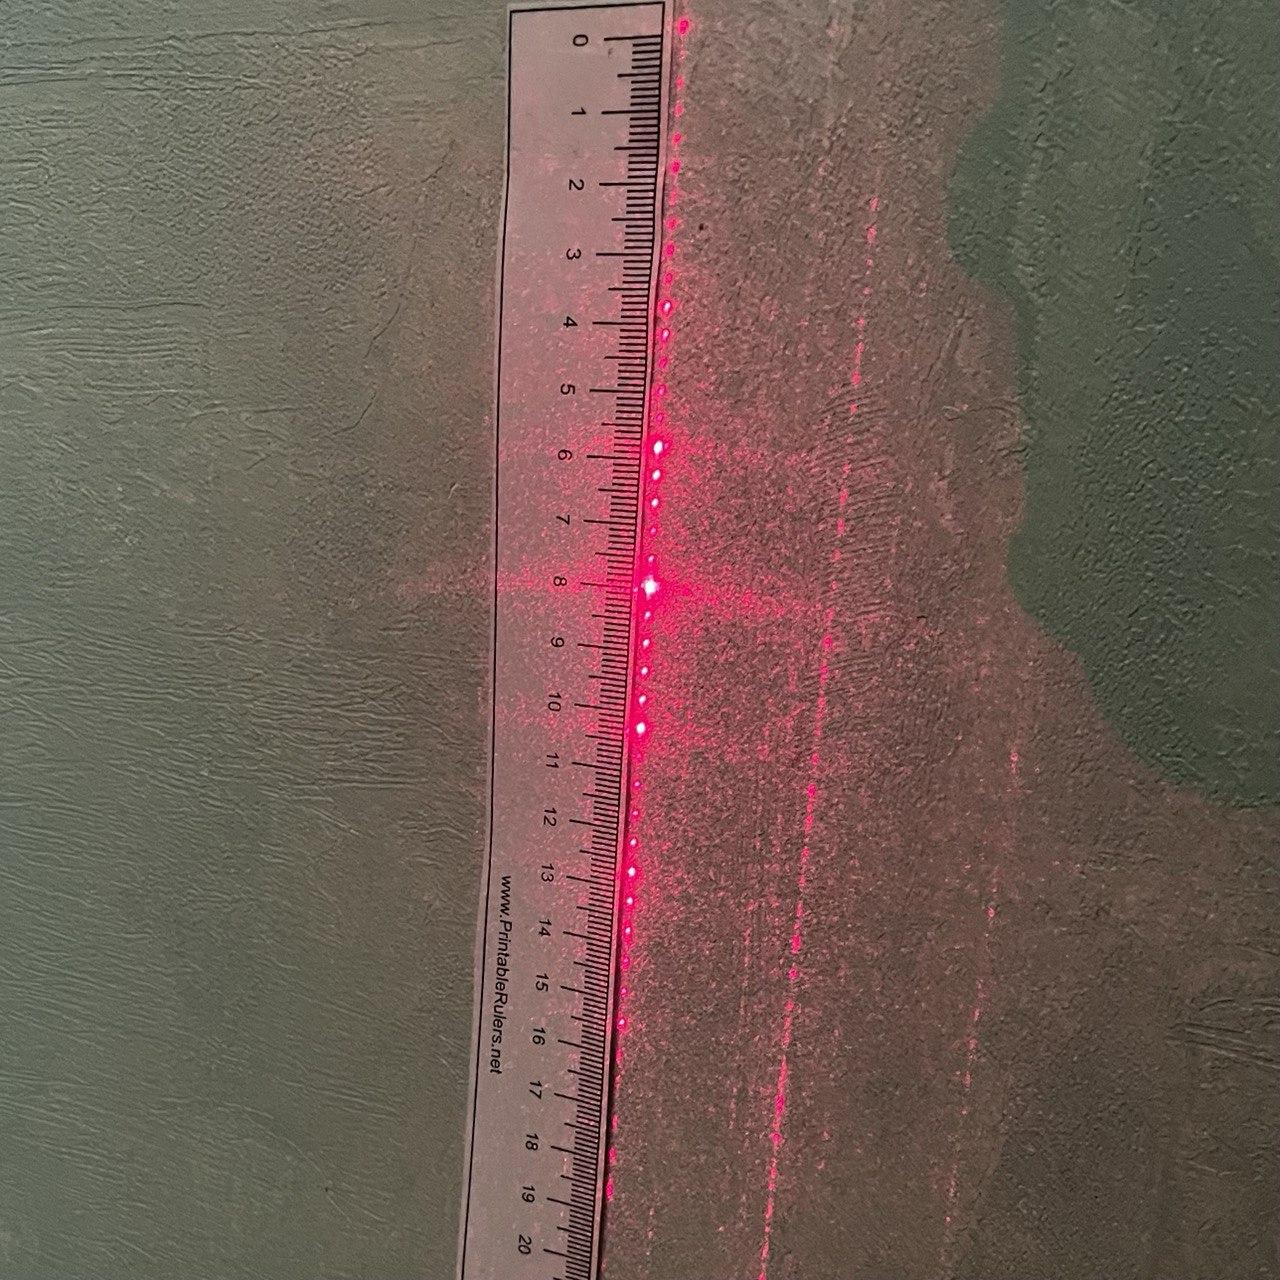
\includegraphics[width=10cm]{ex3.jpg}
    \caption{Дифракционная картина решётки с d = 0.1 мм, n = 5}
    \label{fig:}
  \end{center}
\end{figure}


  \begin{figure}[H]
  \begin{center}
    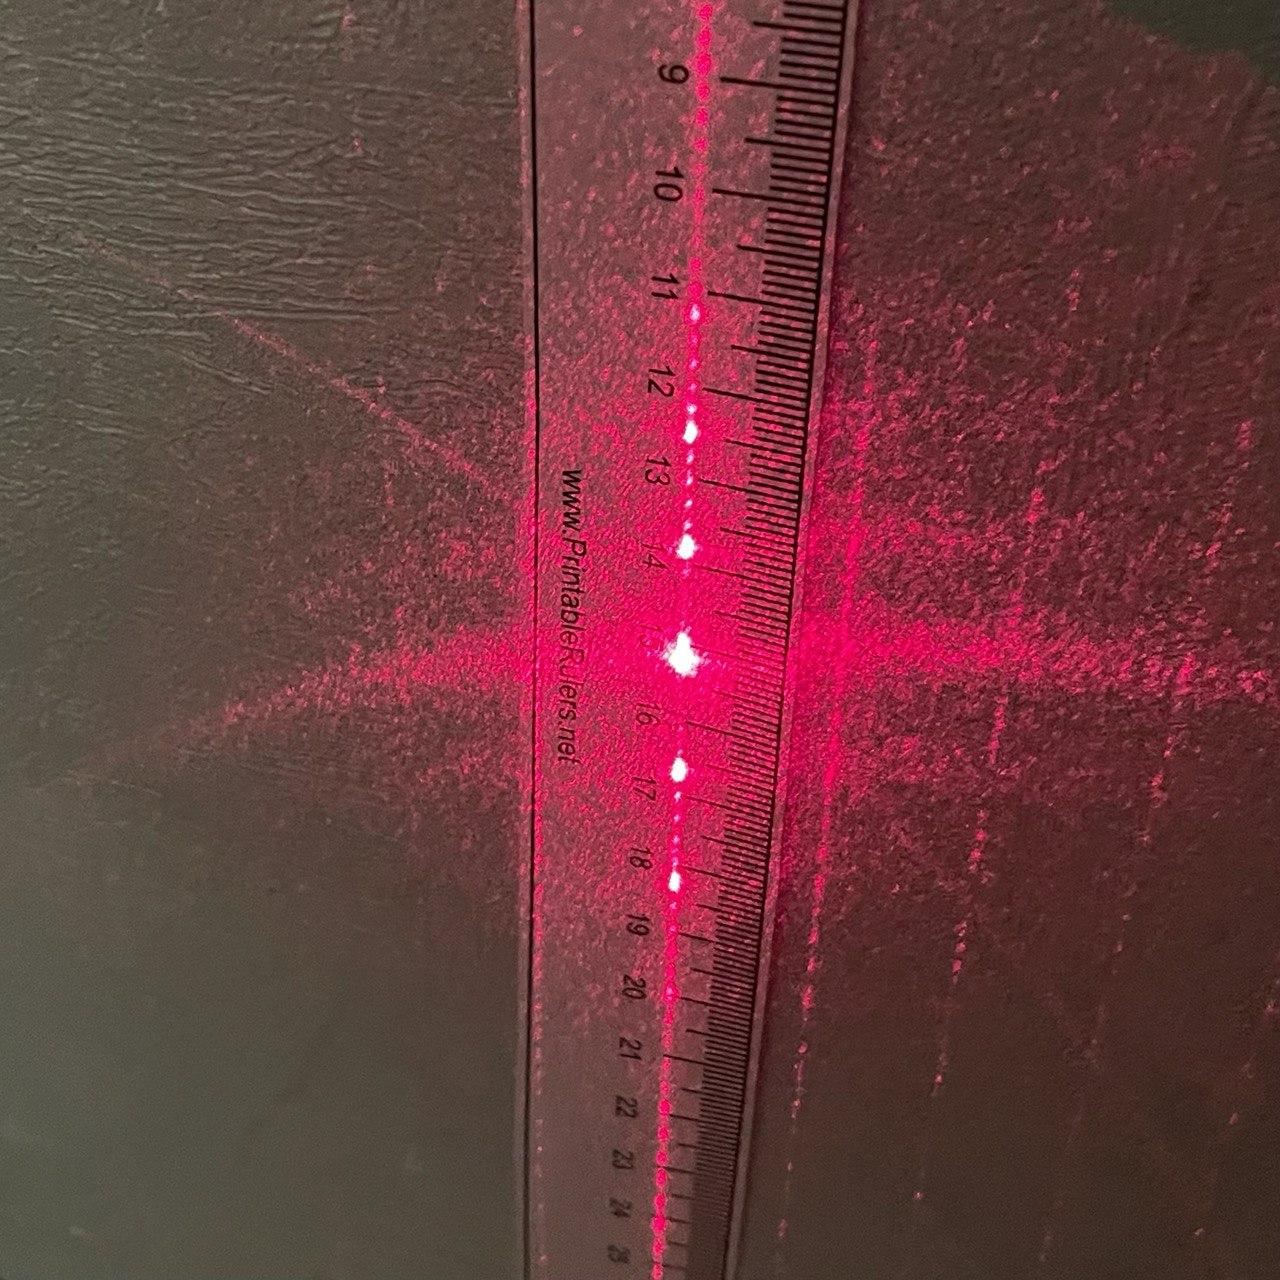
\includegraphics[width=10cm]{ex4.jpg}
    \caption{Дифракционная картина решётки с d = 0.2 мм, n = 5}
    \label{fig:}
  \end{center}
\end{figure}


\item Дифракционная решетка с пятью штрихами на миллиметр и смещением каждого третьего штриха на 0.02 мм дает дифракционную картину изображенную на рис.6. Расстояния между главными максимумами не изменились, но между каждыми соседними максимумами теперь ярко выражены еще 2 максимума, что говорит о наблюдении духа Лаймана с длиной волны $\frac{\lambda}{3}$ и подтвержает теорию.




  \begin{figure}[H]
  \begin{center}
    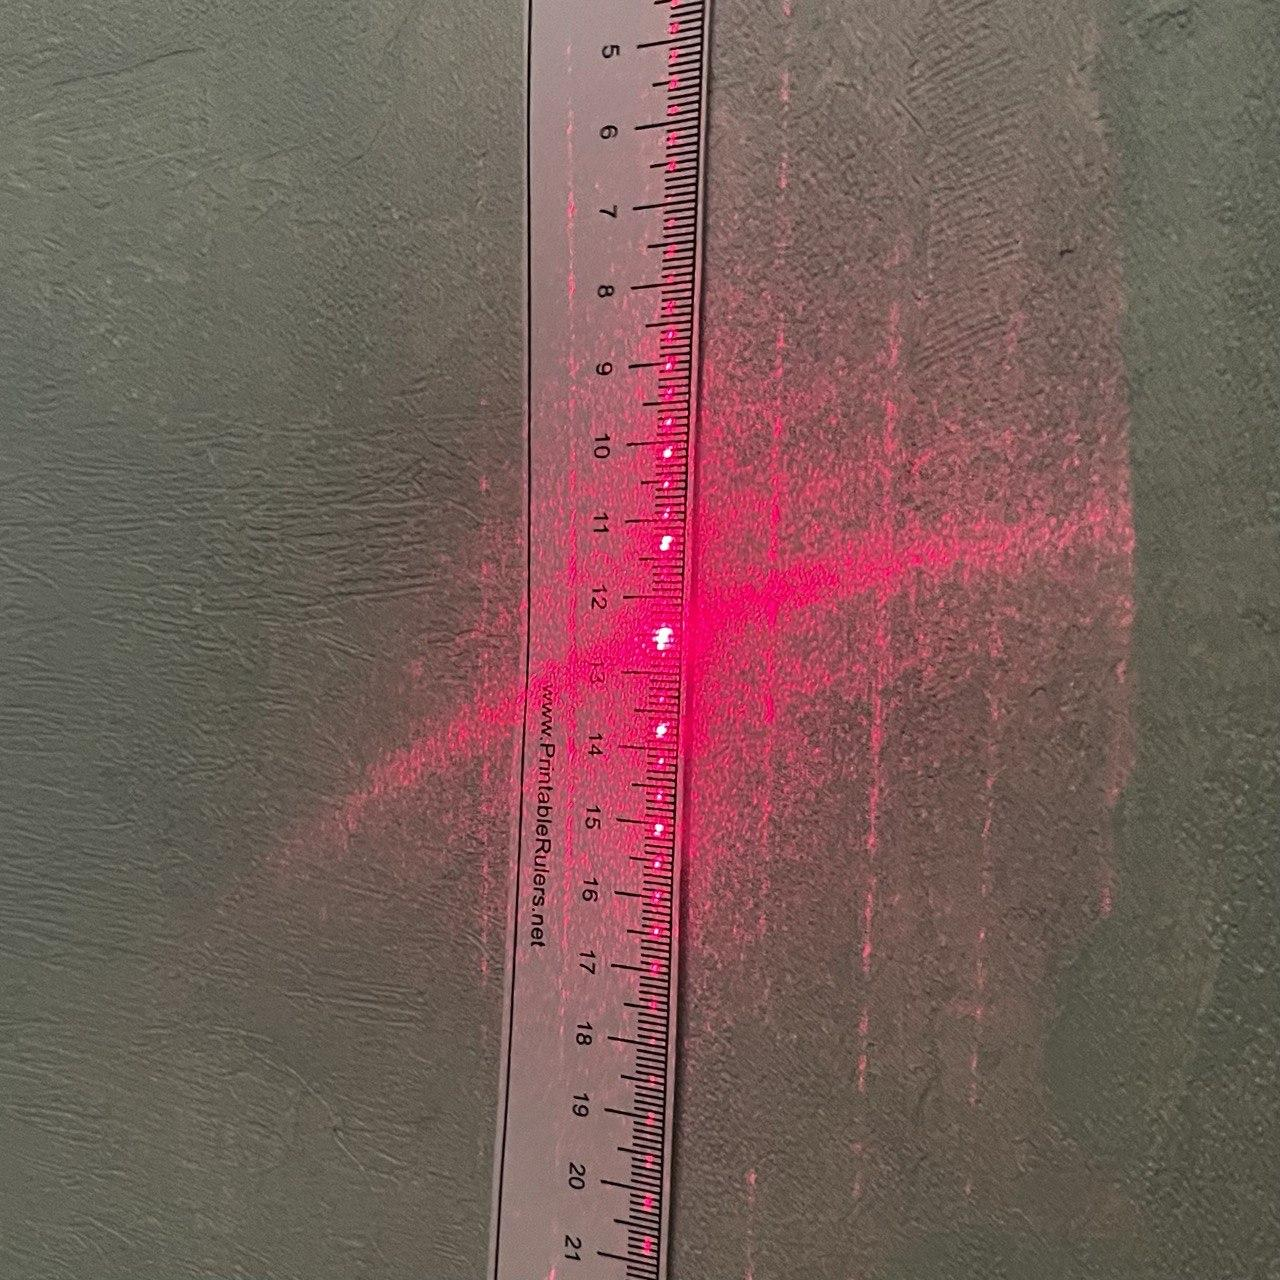
\includegraphics[width=10cm]{ex5.jpg}
    \caption{Дифракционная картина решётки с d = 0.2 мм, n = 3}
    \label{fig:}
  \end{center}
\end{figure}

\item Дифракционные решетки со смещением х = 0.01 мм не дали видимых результатов возникновения ярко выраженных ложных максимумов, что, вероятно, связано с большим периодом и слишком малым смещением. В этих наблюдениях дифракционная картина была смазанной.


\end{enumerate}


\section{Выводы}

В данной работе мы объяснили причину возникновения ложных спектральных линий (духов Лаймана) при дифракции на неточных решетках. Для наблюдения этого эффекта были сделаны дифракционные решетки с периодически повторяющейся ошибкой и произведена дифракция лазерного излучения на них. В эксперименте для двух дифракционных решеток с различными периодами были обнаружены ложные спектральные линии с длиной волны $\frac{\lambda}{5}$ (для периодичности ошибки - n = 5) и $\frac{\lambda}{3}$ (для n = 3), что подтвердило теорию.

$\newline$


\end{document}
	
